
The relative rates for production of different heavy flavor species depend on each
generator's choice of hadronization model and the values of the tunable parameters of that model.
These production fractions have been studied for weakly decaying bottom and charm hadrons in both the \ttbar\
and the high \pT\ jet samples. Results for the \ttbar\ are shown here; the difference between
production fractions in the two processes is less than  0.006.

Figure~\ref{fig:prodfrac} compares the
production fractions for weakly decaying bottom and charm hadrons:

\begin{eqnarray*}
B^{0}\; B^{+}\; B_{s}^{0}\; B_{c}^{+}\; \Lambda_{b}^{0}\; \Xi_{b}^{-}\; \Xi_{b}^{0}\; \Omega_{b}\; D^{+}\; D^{0}\; D_{s}^{+}\; \Lambda_{c}^{+}\; \Xi_{c}^{+}\; \Xi_{c}^{0}\; \Omega_{c}^{0}
\end{eqnarray*} 

\noindent
and their charge conjugates for the four generators.
%in \PythiaE\, \Pythia\, \Herwigpp\ and \Herwig. 
Charm hadron production fractions include only those hadrons produced directly (not from bottom hadron decays).
Although the $\Sigma_B$ should not decay weakly, 
\Herwig\ erroneously decays them weakly under some conditions; these decays are shown on the plot. 
%Differences between the generators are as large as  5-10\%.

%Production fractions for bottom hadrons have larger uncertainties than those for charm hadrons,
%due in part to uncertainties in the baryon fractions.
Recent results from LHCb constrain the ratio of $B_s$ production to $B^0$ production to be
$f_s/f_d = 0.259 \pm 0.015$~\cite{lhcbfsfb}, with no evidence of dependence 
on the \pT\ or $\eta$ of the hadrons.
%LHCb also constrains the ratio of the $\Lambda_B$ baryon to light be
However, the baryon fraction in the forward region is observed to depend significantly on the  
\pT\ and $\eta$ of the hadron~\cite{lhcblam}.  Thus, results from LHCb are of limited use in
constraining baryon production at central rapidities. 

%%which is independent of $f_{\Lambda_B}/(f_u+f_d)= 0.404\pm (0017(stat)\pm0.027(syst)\pm0.105(BR))$. 
The PDG~\cite{PhysRevD.86.010001} provides values for the bottom hadron production fractions at high energy, 

using results obtained from  $Z$ decays and central $p\overline p $ collisions, under the
assumption that these fractions should be universal aside from forward, leading-particle effects
in hadron collisions.
Fractions obtained from the four generators are compared to the PDG values
in Table~\ref{t:bfractions}.
All the generators are in reasonable agreement with the data, although the baryon
fraction in  \PythiaE\ is low.  

For the case of charm hadrons, the experimental data have been
compiled and averaged, including a careful treatment of 
correlated systematic uncertainties in Reference~\cite{r:ffrac}.
Results for the different generators are compared to these averages
in Table~\ref{t:cfractions}.
In general, the generators overestimate the $D^+$ fraction. The $D^0$ fraction
in \Herwig\ is significantly lower than the fraction in the data and other three generators.
Charm baryon fractions 
are poorly constrained by the data and vary widely among the generators.
%These differences in production fractions
%will directly affect the predicted rate for a charm hadron to be tagged as a bottom hadron because the different charm species have significantly different
%lifetimes and semileptonic branching fractions.
%should be give the hadron fractions....right?


\begin{figure}
\centering
\begin{subfigure}[]{0.45\textwidth}
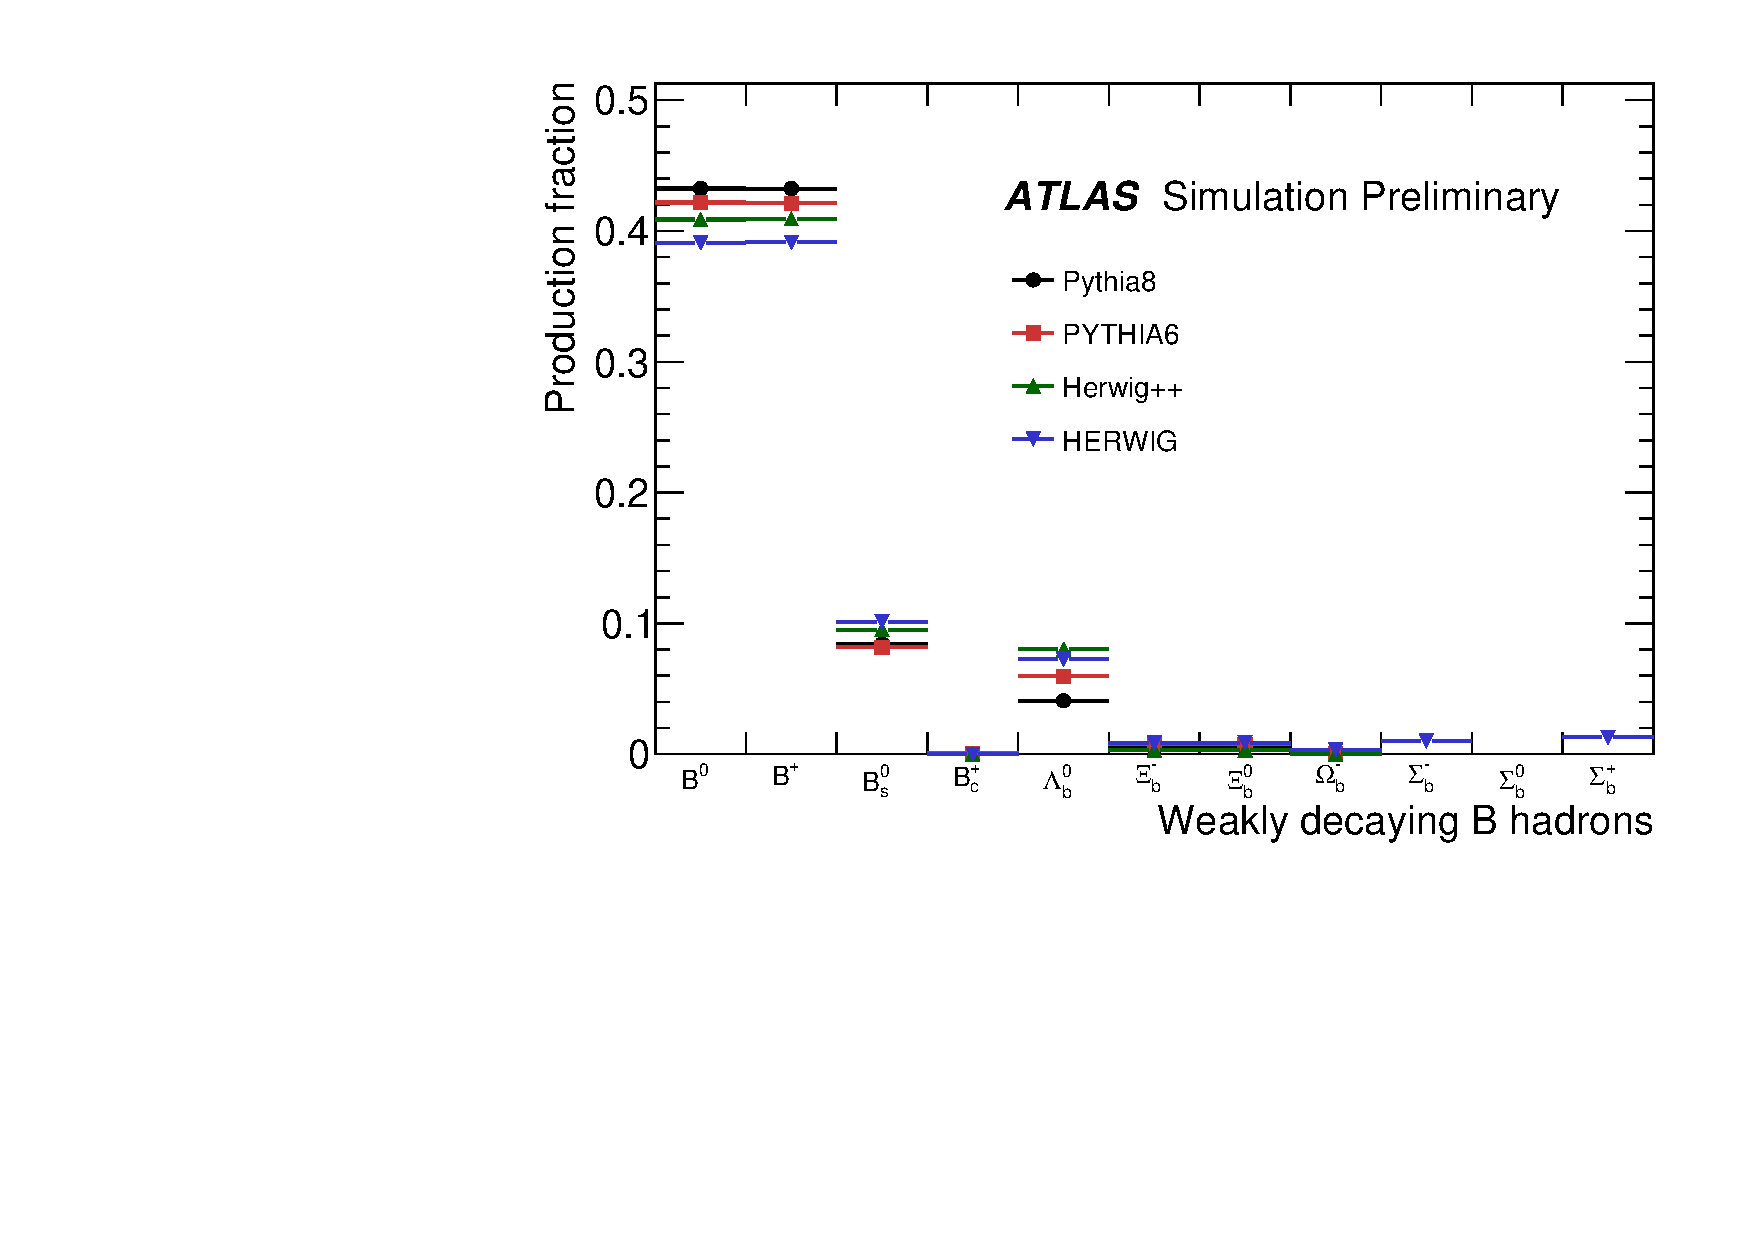
\includegraphics[width=\textwidth]{evtgen/figures/EvtGen/h_bgroundtype.pdf}
\end{subfigure}
\begin{subfigure}[]{0.45\textwidth}
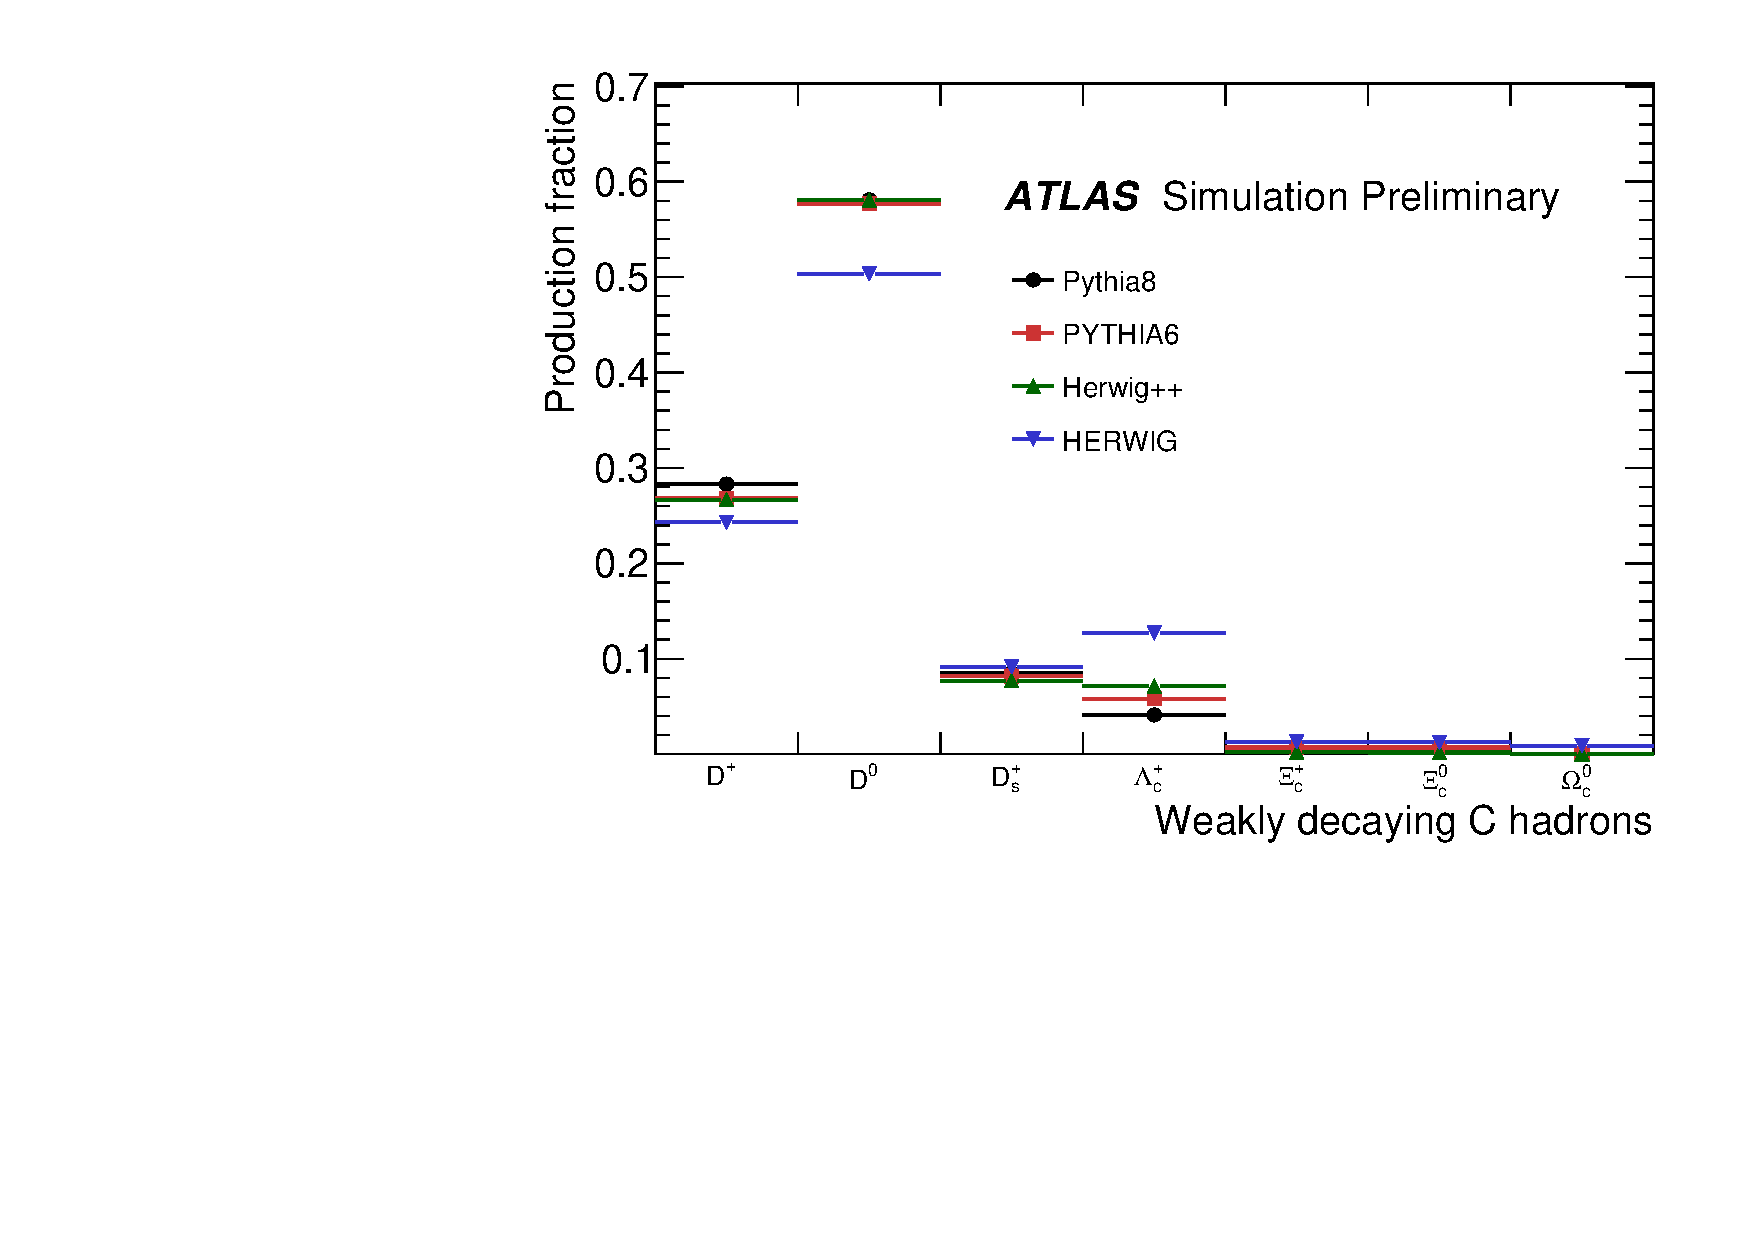
\includegraphics[width=\textwidth]{evtgen/figures/EvtGen/h_cgroundtype.pdf}
\end{subfigure}
\caption{Comparison of the production fractions for various 
weakly decaying (a) bottom and (b) charm hadrons in 
\PythiaE, \Pythia, \Herwigpp\  and \Herwig.
The $\Sigma_{b}$ should not decay weakly, but some weak decays of the $\Sigma_{b}$ are observed in 
\Herwig. 
%The generators disagree as much as 5-10\%, but the baryon fractions are not well known experimentally
}
\label{fig:prodfrac}
\end{figure}


\begin{table}
\begin{center}
\begin{tabular}{|r|r|r|r|r|r|}
\hline
Species &  \PythiaE & \Pythia & \Herwigpp & \Herwig  &  World Average\cite{PhysRevD.86.010001} \\ 
\hline 
$B^+$ &43.2 & 42.1 & 40.9 & 39.1 &   40.2 $\pm$ 0.7  \\
$B^0$  & 43.2 & 42.2 & 40.9 & 39.1 & 40.2 $\pm$ 0.7 \\
$B_s^0$ &8.4 & 8.2 & 9.5 & 10.1 &  10.4 $\pm$ 0.6\\
%$\Lambda_b^0$ & 0.0715733 & 0.0745682 & 0.0506705 & 0.0416447 & 0.08 \\
Baryons &5.1 & 7.3 & 8.6 & 11.7 &  9.3 $\pm$ 1.5\\
\hline
\end{tabular}
\caption{Percentage probability that a bottom quark decays to a bottom
hadron of a given species 
for \PythiaE, \Pythia, \Herwigpp, \Herwig\
and for the world average from Reference~\cite{PhysRevD.86.010001}.}
\label{t:bfractions}
\end{center}%
\end{table}

\begin{table}
\begin{center}
\begin{tabular}{|r|r|r|r|r|r|}
\hline
Species &  \PythiaE & \Pythia & \Herwigpp & \Herwig  & Reference~\cite{r:ffrac}\\
\hline
$D^+$ & 28.3 & 26.8 & 26.7 & 24.3 & 22.56 $\pm$ 0.77\\
$D^0$ & 58.1 & 57.7 & 58.1 & 50.3 & 56.43 $\pm$ 1.51  \\
$D_s$ & 8.5 & 8.2 & 7.7 & 9.2  & 7.97 $\pm$ 0.45\\
Baryons &5.1 & 7.2 & 7.6 & 16.2  & $10.8\pm 0.91$\\
\hline
\end{tabular}
\end{center}%
\caption{Percentage probability that a charm quark fragments to a charmed
hadron of a given species 
%for various Monte Carlo generators
for \PythiaE, \Pythia, \Herwigpp, \Herwig\
and for the world average from Reference~\cite{r:ffrac}.
%The world average baryon fraction is 
%obtained by imposing the constraint that the charm fractions add up to 1.
}
\label{t:cfractions}
\end{table}
